\section{Neuronas adaptativas lineales y la convergencia del entrenamiento}
La neurona adaptativa lineal (\textbf{Adaline}) fué publicada unos años
después del algoritmo del perceptrón de Frank Rosenblatt, por Bernard
Widrow y es considerada un ¿improvement' sobre el perceptrón.
El algoritmo de Adaline es particularmente interesante porque ilustra
el concepto clave de definir y minimizar funciones de costo, lo que
sienta las bases para algoritmos mas avanzados de clasificación,
como la regresión logística o las máquinas de vectores de apoyo.

La principal diferencia entre las reglas de Adaline (también llamada
de \textit{Widrow-Hoff}) y la del perceptrón de Rosenblatt es que los
pesos son actualizados con base en una función de activación lineal,
en lugar de una función escalón. En Adaline, esta función de activación
$\phi (z)$ es simplemente la función identidad de la entrada neta, así
$\phi (w^T x) = w^T x$.

Mientras que la función de activación lineal es usada para la actualiza-
ción de pesos, un \textit{cuantificador}, similar a la función escalón
descrita anteriormente, puede ser usado para hacer la clasificación,
como se ilustra en la siguiente imágen:

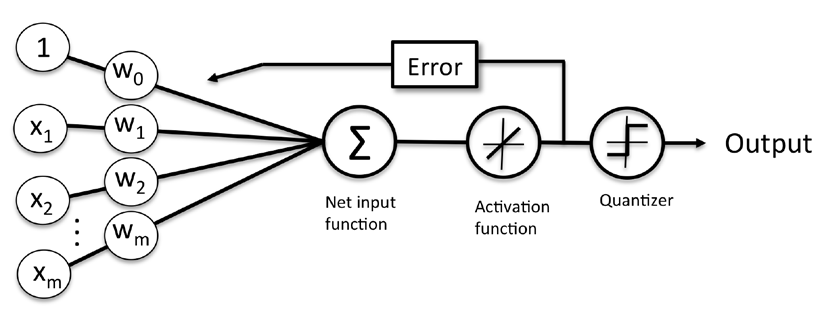
\includegraphics[scale=0.5]{adaline}

Si se compara la imágen anterior con la ilustración del algoritmo del
perceptrón, la diferencia es que se usa la salida con valores continuos
de la función lineal de activación para calcular el error y actualizar
los pesos, en lugar de hacer una clasificación binaria.
